
\phantomsection

% Increment the chapter counter so \thechapter shows the correct number
% and make it referenceable with \ref
\refstepcounter{chapter}

% Manually add this appendix to the Table of Contents
\addcontentsline{toc}{chapter}{Apéndice \thechapter: Búsqueda en bases de datos}

% Add vertical space above the title (mimics standard chapter spacing)
\vspace{40pt}

% Display the actual chapter title (centered, large, bold)
{\centering \normalfont\huge\bfseries Apéndice~\thechapter: Búsqueda en bases de datos~\par}

% Add spacing between title and horizontal rule
\vspace{10pt}

% Draw a horizontal line across the page for visual separation
{\centering \rule{\textwidth}{0.4pt} \par}

% Add vertical space between title section and content
\vspace{40pt}

% Set the running headers for left and right pages
\markboth{Apéndice \thechapter:Búsqueda en bases de datos}{Apéndice \thechapter: Búsqueda en bases de datos}


\section{Búsqueda de artículos sin criterios de inclusión/exclusión}\label{sec:busqueda-sin-criterios}

% ##### Imagenes de busqueda ########

\begin{figure}[H]
	\centering
	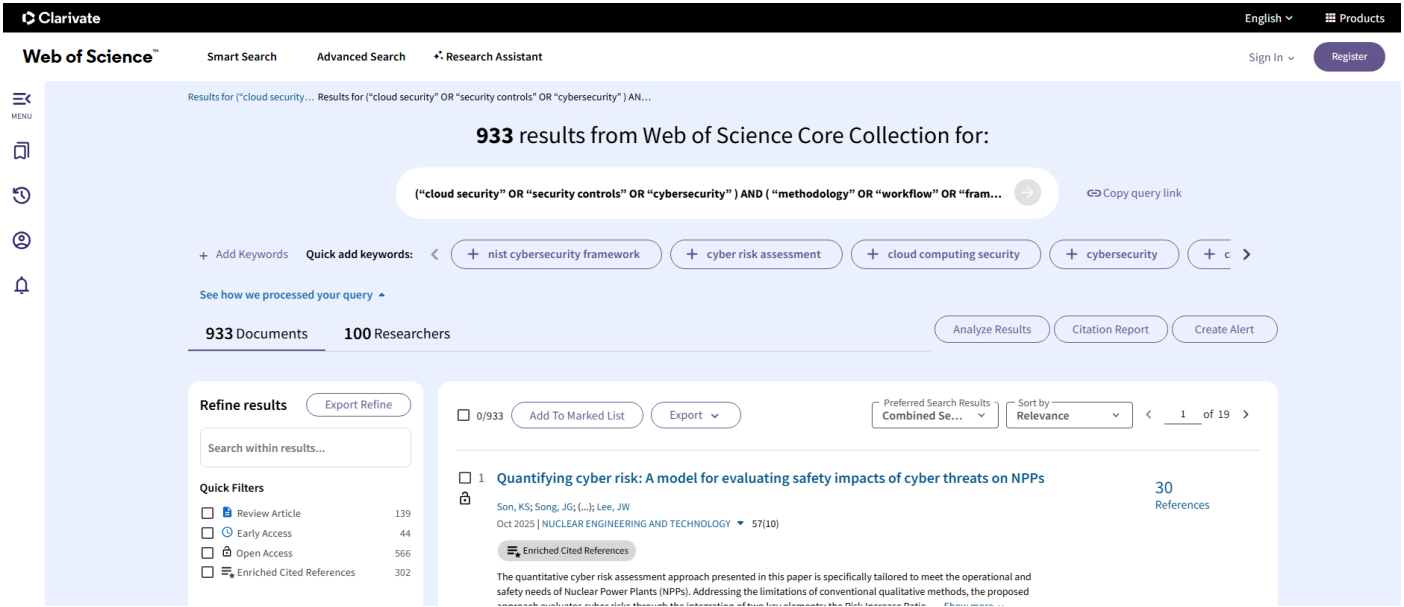
\includegraphics[width=\textwidth,keepaspectratio]{apendices/bases-datos/sin-exclusion/wos.png}
	\caption{Búsqueda de artículos de educación en WOS sin criterios de inclusión/exclusión \\
		Fecha de acceso: 22/01/2026 8:17 pm
	}\label{fig:busqueda-acm-no-exclusion}
\end{figure}

\FloatBarrier

\begin{figure}[H]
	\centering
	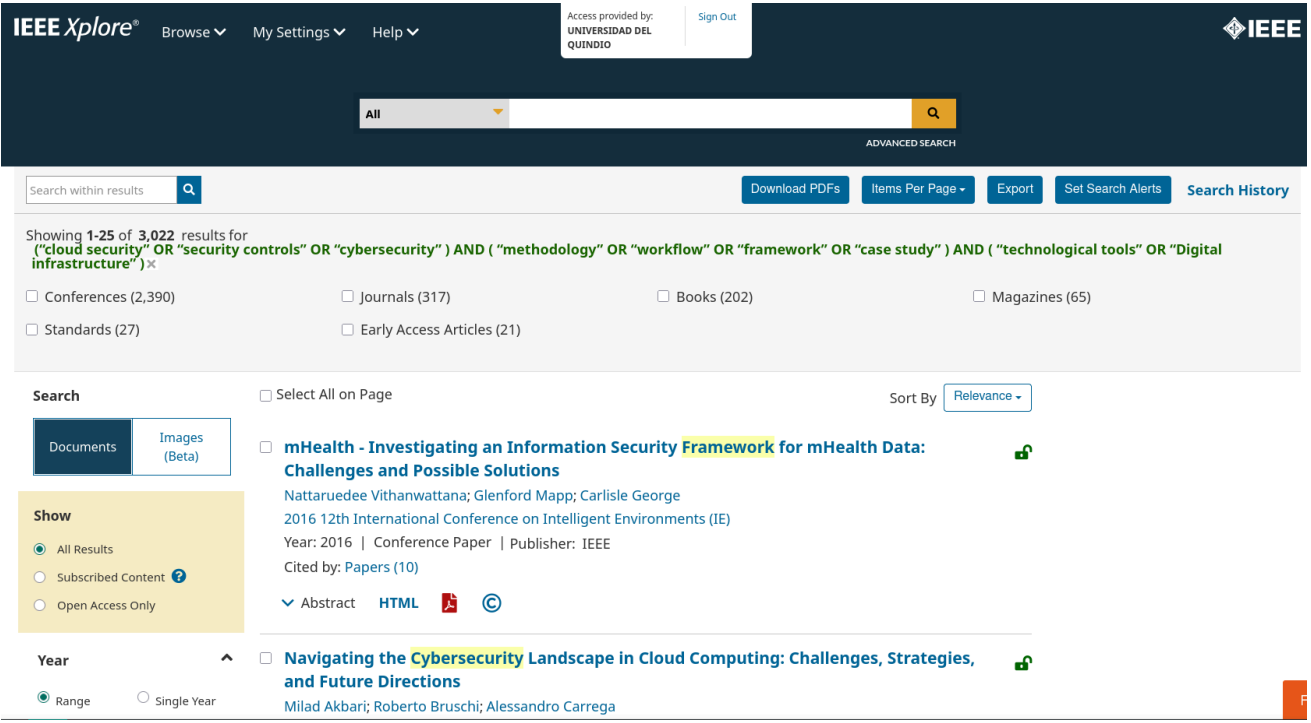
\includegraphics[width=\textwidth,keepaspectratio]{apendices/bases-datos/sin-exclusion/ieee.png}
	\caption{Búsqueda de artículos de investigación en IEEE sin criterios de inclusión/exclusión \\
		Fecha de acceso: 22/01/2026 8:20 pm
	}\label{fig:busqueda-ieee-no-exclusion}
\end{figure}

\begin{figure}[H]
	\centering
	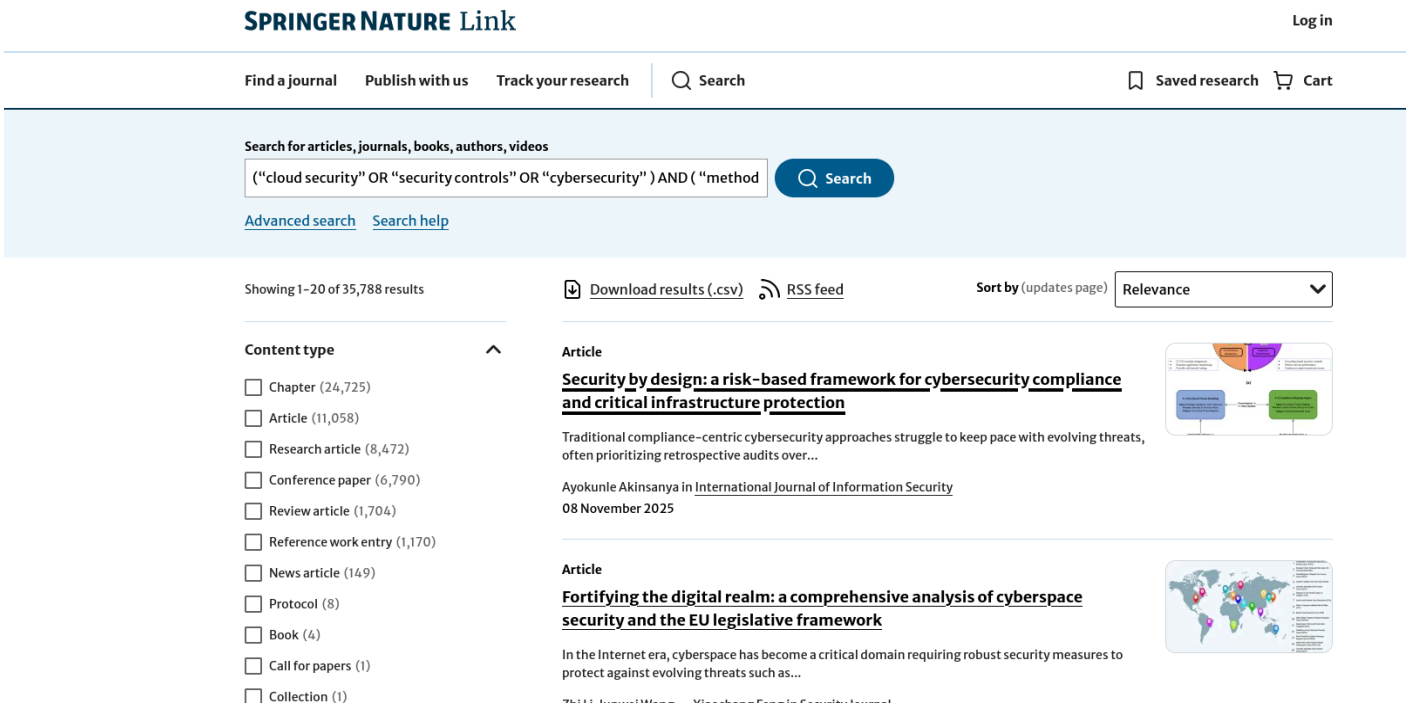
\includegraphics[width=\textwidth,keepaspectratio]{apendices/bases-datos/sin-exclusion/springer.png}
	\caption{Búsqueda de artículos de investigación en Springer sin criterios de inclusión/exclusión \\
		Fecha de acceso: 22/01/2026 8:23 pm
	}\label{fig:busqueda-springer-no-exclusion}
\end{figure}

\begin{figure}[H]
	\centering
	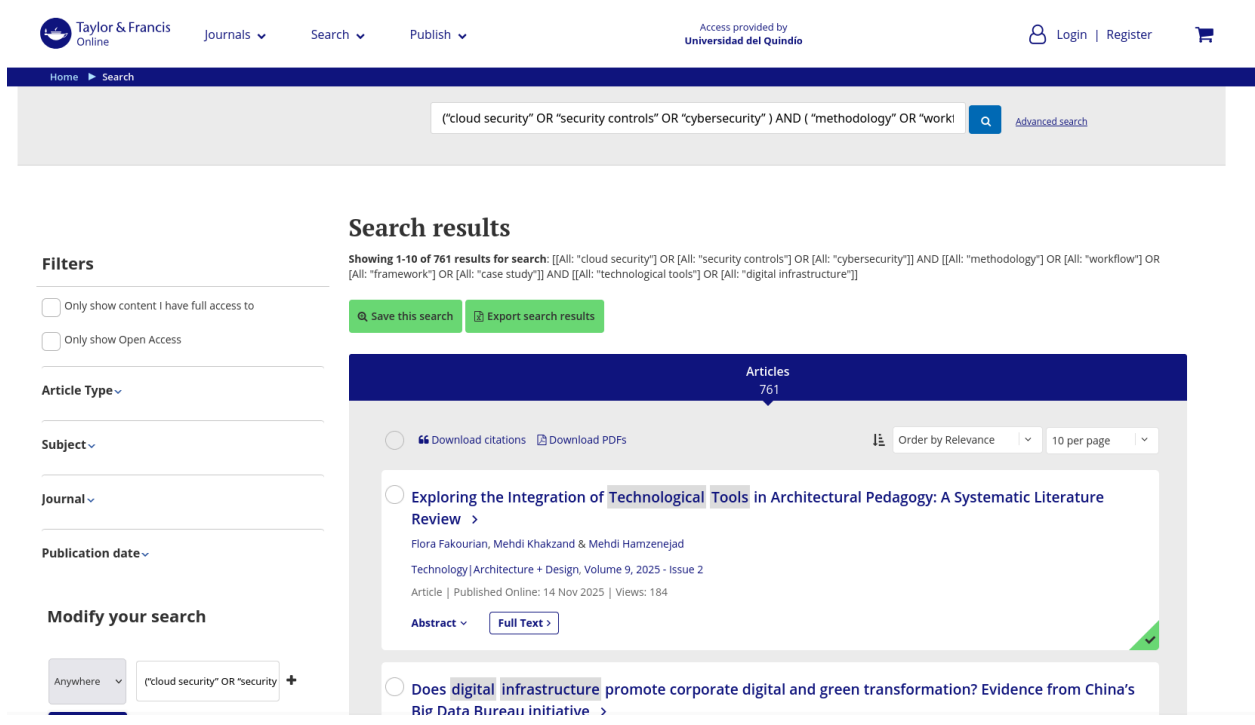
\includegraphics[width=\textwidth,keepaspectratio]{apendices/bases-datos/sin-exclusion/taylor&francis.png}
	\caption{Búsqueda de artículos de investigación en Taylor \& Francis sin criterios de inclusión/exclusión \\
		Fecha de acceso: 22/01/2026 8:25 pm
	}\label{fig:busqueda-taylor-no-exclusion}
\end{figure}

\begin{figure}[H]
	\centering
	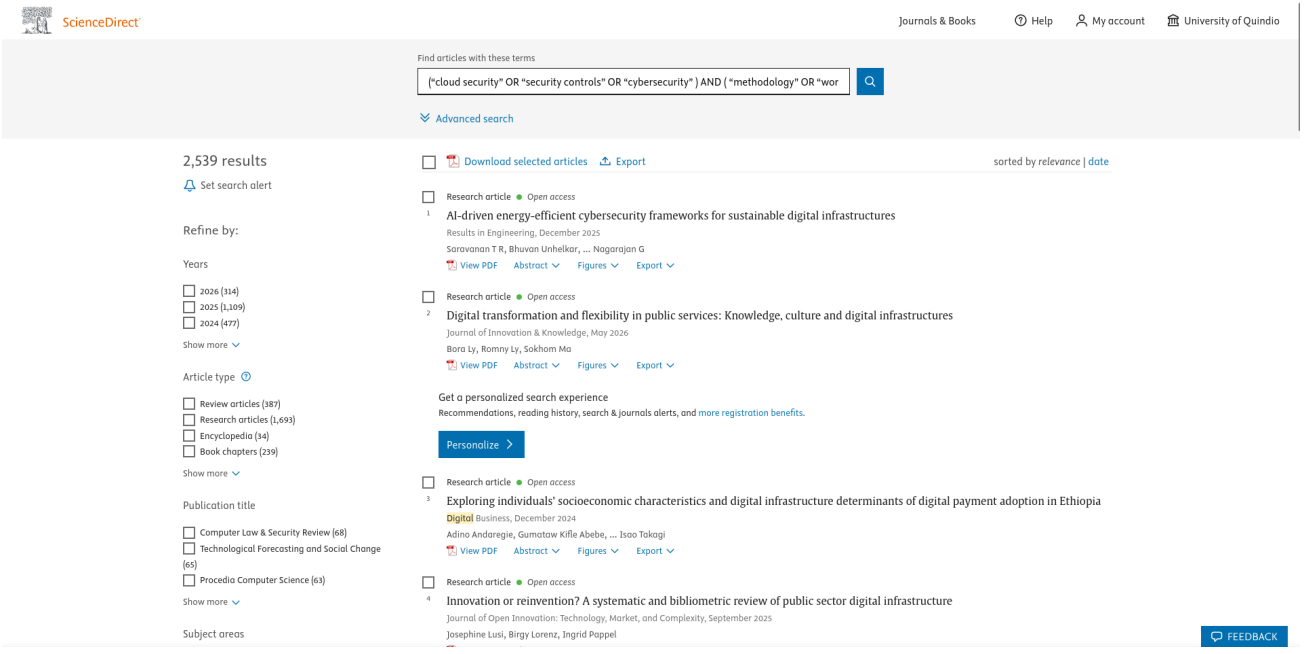
\includegraphics[width=\textwidth,keepaspectratio]{apendices/bases-datos/sin-exclusion/science.png}
	\caption{Búsqueda de artículos de investigación en Science Direct sin criterios de inclusión/exclusión \\
		Fecha de acceso:  22/01/2026 8:28 pm
	}\label{fig:busqueda-science-no-exclusion}
\end{figure}


%########## Fin Imagenes %###################


\section{Búsqueda de artículos con criterios de inclusión/exclusión}\label{sec:busqueda-con-criterios}

\begin{figure}[H]
	\centering
	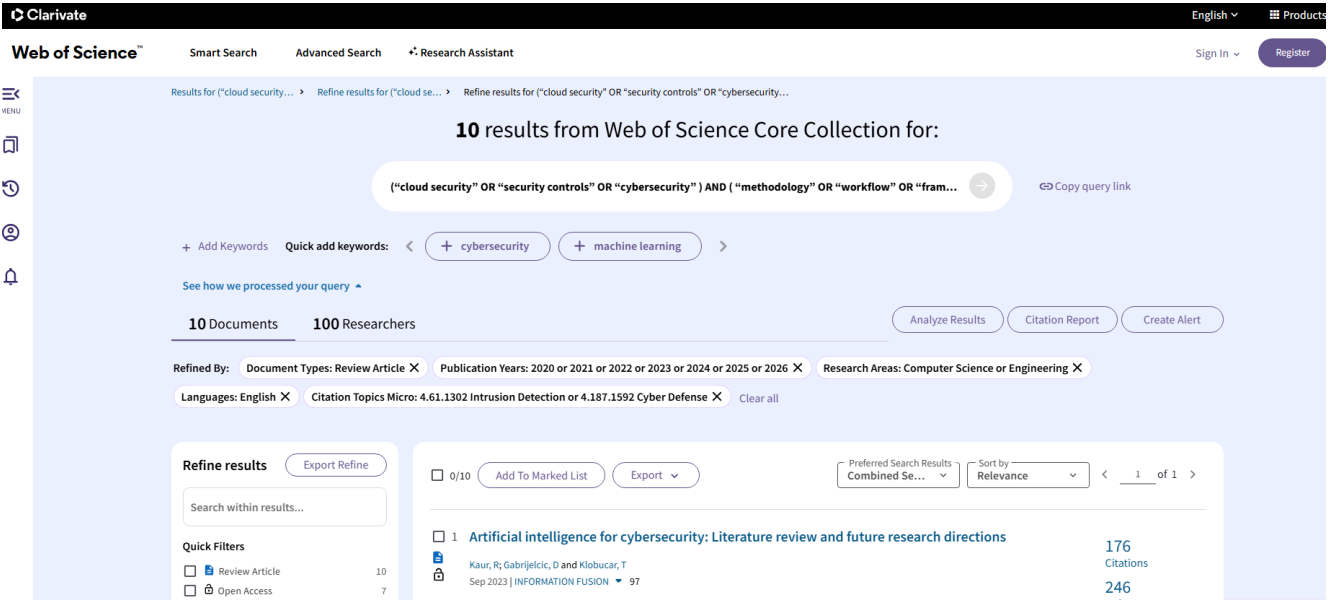
\includegraphics[width=\textwidth,keepaspectratio]{apendices/bases-datos/con-exclusion/wos2.png}
	\caption{Búsqueda de artículos de educación en WOS con criterios de inclusión/exclusión \\
		Fecha de acceso: 22/01/2026 8:55 pm
	}\label{fig:busqueda-wos-con-exclusion}
\end{figure}

\FloatBarrier

\begin{figure}[H]
	\centering
	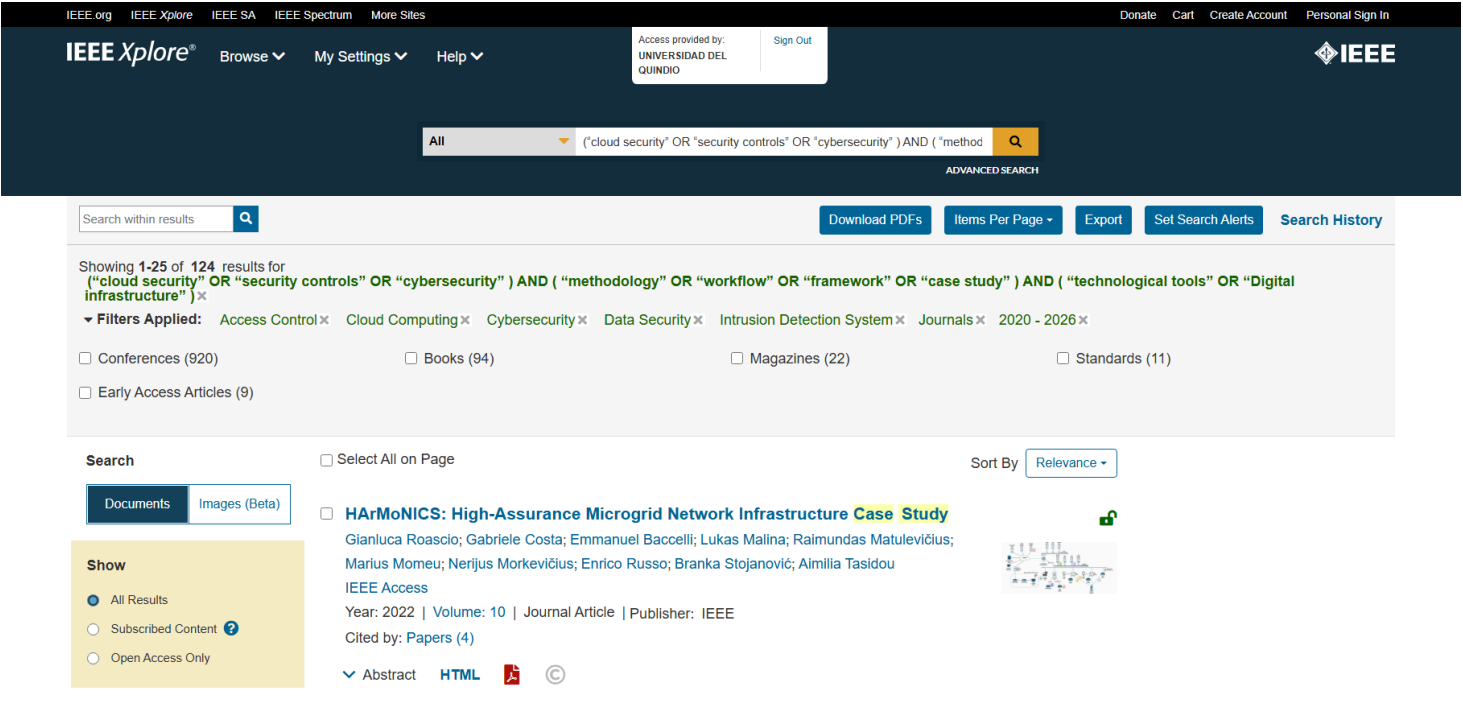
\includegraphics[width=\textwidth,keepaspectratio]{apendices/bases-datos/con-exclusion/ieee2.png}
	\caption{Búsqueda de artículos de investigación en IEEE con criterios de inclusión/exclusión \\
		Fecha de acceso: 22/01/2026 9:00 pm
	}\label{fig:busqueda-ieee-con-exclusion}
\end{figure}

\begin{figure}[H]
	\centering
	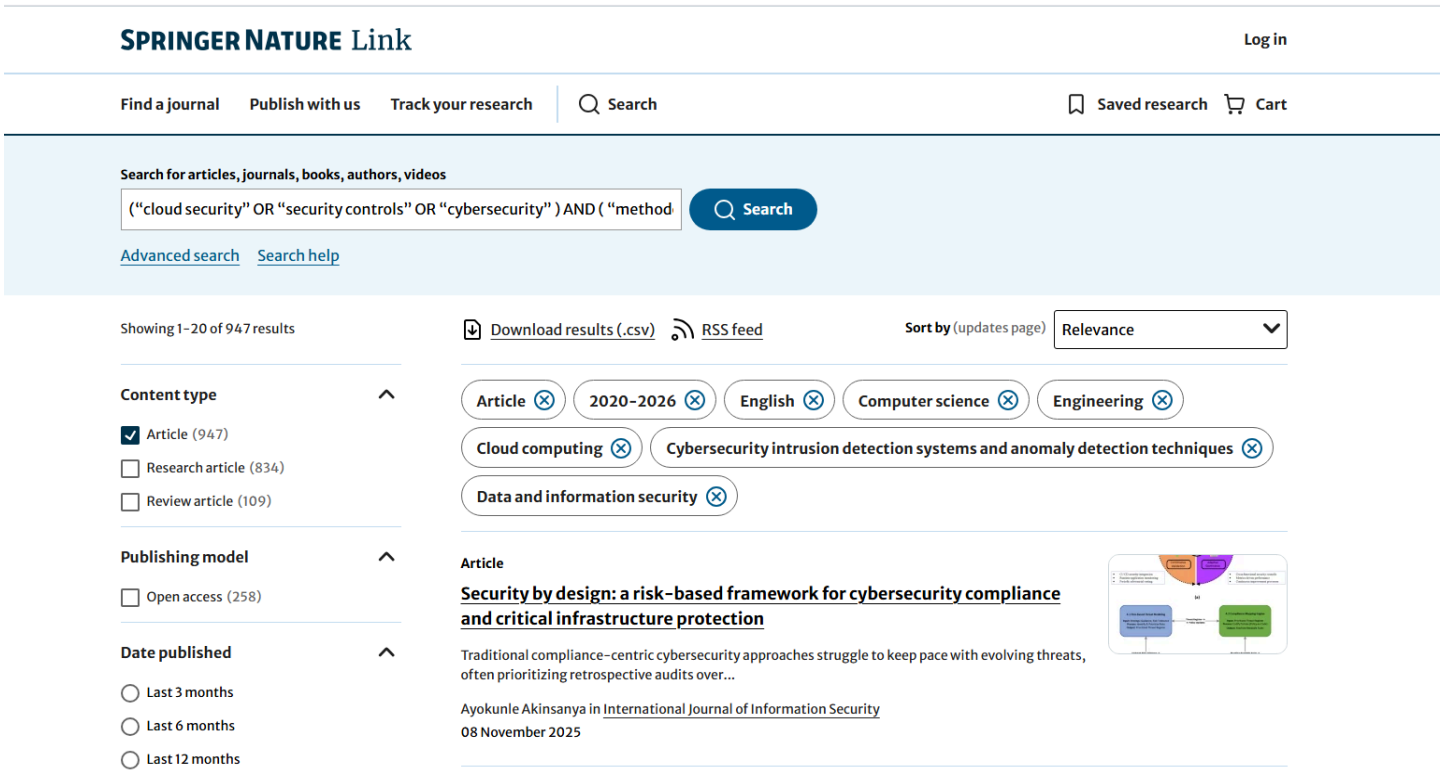
\includegraphics[width=\textwidth,keepaspectratio]{apendices/bases-datos/con-exclusion/springer2.png}
	\caption{Búsqueda de artículos de investigación en Springer con criterios de inclusión/exclusión \\
		Fecha de acceso: 22/01/2026 9:07 pm
	}\label{fig:busqueda-springer-con-exclusion}
\end{figure}

\begin{figure}[H]
	\centering
	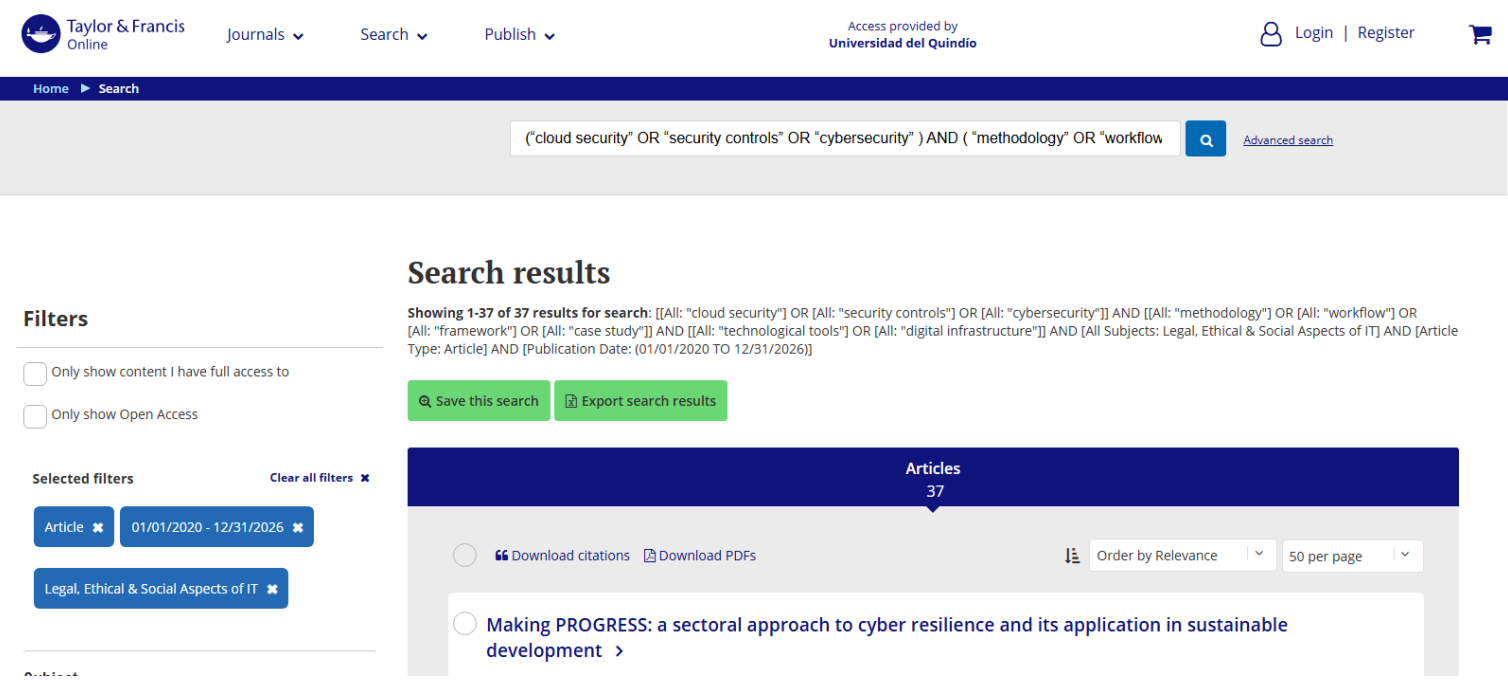
\includegraphics[width=\textwidth,keepaspectratio]{apendices/bases-datos/con-exclusion/taylor&francis2.png}
	\caption{Búsqueda de artículos de investigación en Taylor \& Francis con criterios de inclusión/exclusión \\
		Fecha de acceso: 22/01/2026 9:10 pm
	}\label{fig:busqueda-taylor-con-exclusion}
\end{figure}

\begin{figure}[H]
	\centering
	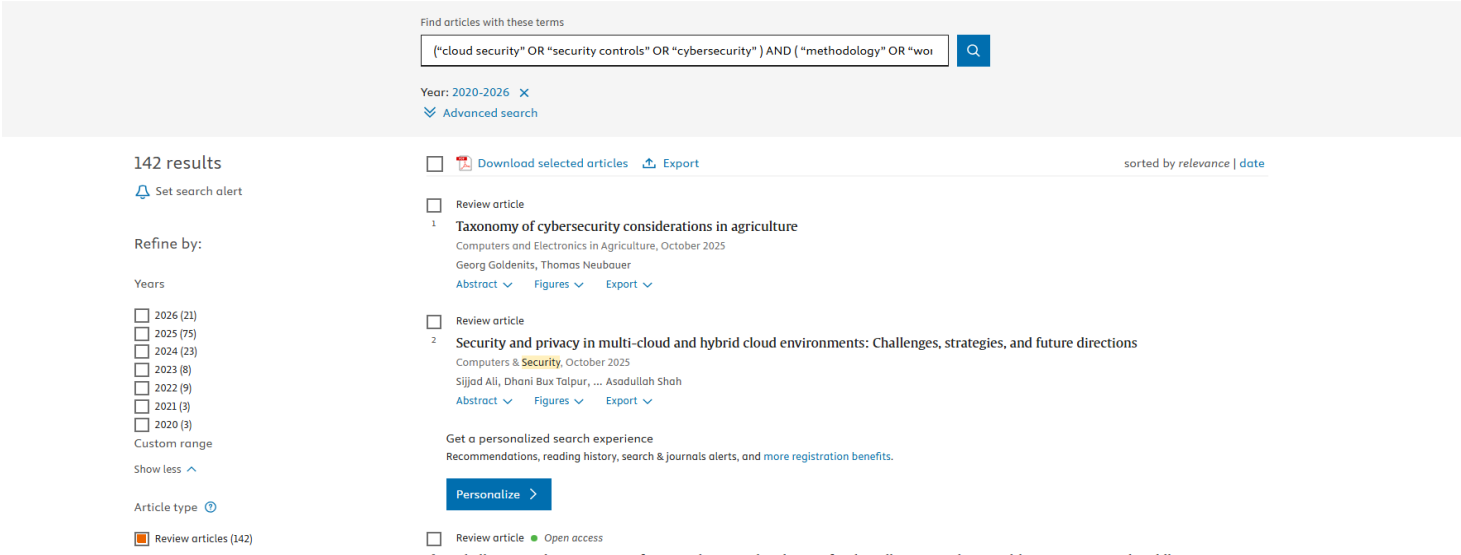
\includegraphics[width=\textwidth,keepaspectratio]{apendices/bases-datos/con-exclusion/science2.png}
	\caption{Búsqueda de artículos de investigación en Science Direct con criterios de inclusión/exclusión \\
		Fecha de acceso: 22/01/2026 9:13 pm
	}\label{fig:busqueda-science-con-exclusion}
\end{figure}